\subsubsection{Boundry-klasse: XboxController}

Denne klasse har til formål at agere API for Xbox Controlleren til PC softwaren. Til dette skal udnyttes standard biblioteket; XInput. Det skal være muligt at få alt det data der udnyttes til at bestemme bilens retning, ved et enkelt funktionskald for simplicitet. På Figur \ref{fig:cd_xboxcontroller} kan ses et klasse diagram over den ønskede klasse efterfulgt af funktionalitet.

\begin{figure}[h]
\centering
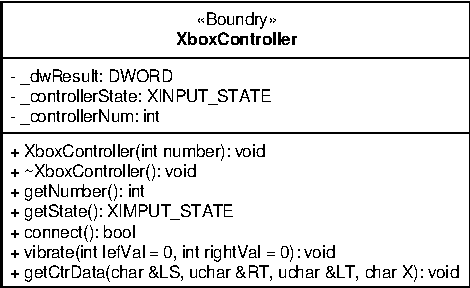
\includegraphics[]{../fig/diagrammer/pc/cd_xboxcontroller.pdf}
\caption{Klassebeskrivelse for boundry-klassen XboxController}
\label{fig:cd_xboxcontroller}
\end{figure}

\textbf{Attributter}

\begin{table}[h]
\begin{tabularx}{\textwidth}{| Z | Z | L{10cm} |} \hline
Navn & Type & Beskrivelse \\\hline
\texttt{\_dwResult}				& \texttt{DWORD}		&Variabel af typen DWORD, skal indeholde data om controllerens tilstand.\\\hline

\texttt{\_controller- State}	& \texttt{XINPUT\_STATE}&Struct af typen XINPUT\_STATE. Indeholder hhv. DWORD, der indeholder en værdi forskellig fra 0 hvis der er sket en ændring i controllerens tilstand, og XINPUT\_GAMEPAD, der indeholder alle værdier som fortæller om controllerens nuværende tilstand.\\\hline

\texttt{\_controller- Num}		& \texttt{int}			&Variabel af typen int der indeholder controller nummer.\\\hline
\end{tabularx}
\caption{Attributter for klassen XboxController}
\label{table:attr_xboxcontroller}
\end{table}

\textbf{Metoder}

\begin{table}[h]
\begin{tabularx}{\textwidth}{| L{2.5 cm} | Z |} \hline
Prototype 	& \texttt{void XboxController(int number)} \\\hline
Parametre 	& \texttt{number} 			\newline Det ønskede controller ID (1-4). \\\hline
Returværdi	& \texttt{void} 			\newline \\\hline
Beskrivelse	& Constructor til klassen XboxController. \newline \\\hline
\end{tabularx}
\caption{Metodebeskrivelse for constructoren af \texttt{XboxController} klassen}
\label{table:met_xboxcontroller}
\end{table}

\clearpage

\begin{table}[h]
\begin{tabularx}{\textwidth}{| L{2.5 cm} | Z |} \hline
Prototype 	& \texttt{void $\sim$XboxController()} \\\hline
Parametre 	& \texttt{void}				\newline \\\hline
Returværdi	& \texttt{void} 			\newline \\\hline
Beskrivelse	& Destructor til klassen XboxController. \newline \\\hline
\end{tabularx}
\caption{Metodebeskrivelse for destructoren af \texttt{XboxController} klassen}
\label{table:met_xboxcontroller_de}
\end{table}

\begin{table}[h]
\begin{tabularx}{\textwidth}{| L{2.5 cm} | Z |} \hline
Prototype 	& \texttt{int getNumber()} \\\hline
Parametre 	& \texttt{void}				\newline \\\hline
Returværdi	& \texttt{int} 				\newline Controllerens ID \\\hline
Beskrivelse	& Denne funktion har til formål at returnere objektets ID. \newline \\\hline
\end{tabularx}
\caption{Metodebeskrivelse for \texttt{getNumber()}}
\label{table:met_getnumber}
\end{table}

\begin{table}[h]
\begin{tabularx}{\textwidth}{| L{2.5 cm} | Z |} \hline
Prototype 	& \texttt{XINPUT\_STATE getState()} \\\hline
Parametre 	& \texttt{void}				\newline \\\hline
Returværdi	& \texttt{XINPUT\_STATE} 	\newline Struct af typen XINPUT\_STATE. Indeholder hhv. DWORD og XINPUT\_GAMEPAD. \\\hline
Beskrivelse	& Denne funktion har til formål at opdatere \_controllerState som indeholder controllerens nuværende tilstand og info om hvorvidt den har skiftet tilstand. \\\hline
\end{tabularx}
\caption{Metodebeskrivelse for \texttt{getState()}}
\label{table:met_getstate}
\end{table}

\begin{table}[h]
\begin{tabularx}{\textwidth}{| L{2.5 cm} | Z |} \hline
Prototype 	& \texttt{bool connect()} \\\hline
Parametre 	& \texttt{void}				\newline \\\hline
Returværdi	& \texttt{bool} 			\newline Controllerens connection tilstand \\\hline
Beskrivelse	&  Denne funktion returnerer hvorvidt der er forbindelse til controlleren. \\\hline
\end{tabularx}
\caption{Metodebeskrivelse for \texttt{connect()}}
\label{table:met_connect}
\end{table}

\clearpage

\begin{table}[h]
\begin{tabularx}{\textwidth}{| L{2.5 cm} | Z |} \hline
Prototype 	& \texttt{void vibrate(int leftVal = 0, int rightVal = 0)} \\\hline
Parametre 	& \texttt{leftVal}			\newline En værdi der fortæller controllerklassen hvor hurtigt vibrater motoren i venstre side af controlleren skal køre (0 - 65535).	\newline \newline
			  \texttt{rightVal}			\newline En værdi der fortæller controllerklassen hvor hurtigt vibrater motoren i højre side af controlleren skal køre (0 - 65535). \\\hline
Returværdi	& \texttt{void} 			\newline \\\hline
Beskrivelse	&  Denne funktion igangsætter højre og venstre vibrater med en styrke alt efter input parameterne leftVal og rightVal. Inputparameterne kan gå mellem 0 og 65535, hvor 0 er ingen vibrering og 65535 er maksimal vibrering. Hvis der ikke gives parametre med i funktionen, vil den automatisk sætte parameterne til 0 og dermed slukke for vibraterne.\\\hline
\end{tabularx}
\caption{Metodebeskrivelse for \texttt{vibrate()}}
\label{table:met_vibrate}
\end{table}

\begin{table}[h]
\begin{tabularx}{\textwidth}{| L{2.5 cm} | Z |} \hline
Prototype 	& \texttt{void getCtrlData(char \&LS, uchar \&RT, uchar \&LT, char X)} \\\hline
Parametre 	& \texttt{LS}				\newline En reference til den char der ønskes at funktionen indsætter data om controllerens ''Left Stick'' tilstand i.				\newline \newline
			  \texttt{RT}				\newline En reference til den unsigned char der ønskes at funktionen indsætter data om controllerens ''Right Trigger'' tilstand i.\newline \newline
			  \texttt{LT}				\newline En reference til den unsigned char der ønskes at funktionen indsætter data om controllerens ''Left Trigger'' tilstand i.\newline \newline
			  \texttt{X}				\newline En reference til den char der ønskes at funktionen indsætter data om controllerens ''X-button'' tilstand i. \\\hline
Returværdi	& \texttt{void} 			\newline \\\hline
Beskrivelse	&  Denne funktion har til formål at returnere nye controller tilstande, for controllerens Left Stick, Right Trigger, Left Trigger og X-button, på de refererede parametres plads.\\\hline
\end{tabularx}
\caption{Metodebeskrivelse for \texttt{getCtrlData()}}
\label{table:met_getctrldata}
\end{table}